% \addtolength{\tabcolsep}{-0.4em}
\renewcommand{\arraystretch}{1} % Default value: 1

\newcommand{\drawborder}[4]{
  \draw[#3,#4] ($(#2.north west)+(-13pt,0pt)$) -- (#2.north east) -- (#2.south east) -| ($(#2.north west)+(-13pt,0pt)$);
}

\makeatletter
\tikzset{
    database/.style={
        path picture={
            \draw (0, 1.5*\database@segmentheight) circle [x radius=\database@radius,y radius=\database@aspectratio*\database@radius];
            \draw (-\database@radius, 0.5*\database@segmentheight) arc [start angle=180,end angle=360,x radius=\database@radius, y radius=\database@aspectratio*\database@radius];
            \draw (-\database@radius,-0.5*\database@segmentheight) arc [start angle=180,end angle=360,x radius=\database@radius, y radius=\database@aspectratio*\database@radius];
            \draw (-\database@radius,1.5*\database@segmentheight) -- ++(0,-3*\database@segmentheight) arc [start angle=180,end angle=360,x radius=\database@radius, y radius=\database@aspectratio*\database@radius] -- ++(0,3*\database@segmentheight);
        },
        minimum width=2*\database@radius + \pgflinewidth,
        minimum height=3*\database@segmentheight + 2*\database@aspectratio*\database@radius + \pgflinewidth,
    },
    database segment height/.store in=\database@segmentheight,
    database radius/.store in=\database@radius,
    database aspect ratio/.store in=\database@aspectratio,
    database segment height=0.1cm,
    database radius=0.25cm,
    database aspect ratio=0.35,
}
\makeatother


\begin{tikzpicture}[node distance=3pt, line width=0.5pt, inner xsep=0.4mm, inner ysep=0.5mm,use Hobby shortcut]
    \sffamily
    \node[draw=argray, fill=arlightgray, inner ysep=0mm, minimum width=178pt, minimum height=100pt,rounded corners=2pt](rewriteengine) {};
    \node[draw=none, fill=none, inner ysep=0mm, below=of rewriteengine.south,yshift=0pt, xshift=0pt](rewriteenginelbl) {\footnotesize{\textbf{Rewrite Engine}}};

    \node[draw=argray!70, fill=white,rounded corners=2pt, inner sep=1mm,below=of rewriteengine.north, yshift=-5pt, xshift=60pt, line width=0.4pt](nfst) {
        \shortstack[c]{
            \texttt{\scriptsize{\textbf{SQL Parse Tree}}} \\[1pt]
            \texttt{\scriptsize{\textbf{(AST)}}}        
        }
        };

    \node[draw=none, fill=white, inner ysep=0mm,right=of nfst, xshift=12pt, yshift=10pt] (wq1){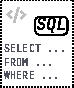
\includegraphics[scale=0.65]{img/fig_SQLDot.pdf}};
    \node[draw=none, fill=white, inner ysep=0mm,right=of nfst, xshift=15pt, yshift=13pt]{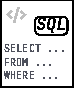
\includegraphics[scale=0.65]{img/fig_SQL.pdf}};
    \node[draw=none, fill=white, inner ysep=0mm,right=of nfst, xshift=18pt, yshift=16pt]{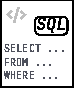
\includegraphics[scale=0.65]{img/fig_SQL.pdf}};
    \node[draw=none, fill=white, inner ysep=0mm,right=of nfst, xshift=21pt, yshift=19pt] (wqm) {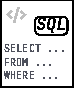
\includegraphics[scale=0.65]{img/fig_SQL.pdf}};

    \node[draw=none, fill=white, inner ysep=0mm,below=of wq1, xshift=0pt, yshift=2pt]{\small{\textsf{Q$_1$, Q$_2$,...}}};


     \node[draw=none, fill=none,left=of nfst, yshift=0pt, xshift=2pt](nfstout) {
        \shortstack[c]{
            \texttt{\scriptsize{internal}} \\[2.5pt]
            \texttt{\scriptsize{representation}}        
        }};

    \node[draw=argray!70, fill=white,rounded corners=2pt, inner sep=1mm,left=of nfst, yshift=0pt, xshift=-48pt, line width=0.4pt](fks) {
        \shortstack[c]{
            \texttt{\scriptsize{\textbf{Extract}}} \\
            \texttt{\scriptsize{\textbf{Fragment Keys}}}        
        }};
    
    \node[draw=argray!70, fill=white,rounded corners=2pt, inner sep=1mm,below=of fks, yshift=-18pt, xshift=0pt, line width=0.4pt, minimum width=50pt, minimum height=50pt](selectedrules) {}; 
    
    \node[draw=arblue, fill=arblue!10, inner ysep=0mm, below=of selectedrules.north,yshift=0pt, xshift=-4pt, minimum width=38pt, minimum height=30pt, line width=0.4pt](rm) {};
    \node[draw=arred, fill=arred!10,  densely dotted,inner ysep=0mm, below=of rm.north,yshift=-4pt, xshift=4pt, minimum width=38pt, minimum height=30pt, line width=0.4pt](rk) {};
    \node[draw=arbluelight, fill=arbluelight!10,inner ysep=0mm, below=of rk.north,yshift=-4pt, xshift=4pt, minimum width=38pt, minimum height=30pt, line width=0.4pt](r1) {};

    \node[draw=none, fill=none,inner sep=1mm,above=of selectedrules.north, yshift=-2pt, xshift=0pt](cadidaterules) {\texttt{\scriptsize{\textbf{Candidate Rules}}}};
       
    \draw[line width=2pt,-{Triangle[width=3*2pt,length=6pt]},draw=argray ] (nfst) -- (fks);     
    \draw[-{Latex[scale=0.8]}, argray] ($(fks.west)+(0pt,6pt)$) -- ($(fks.west)+(-37pt,6pt)$); 
    \draw[-{Latex[scale=0.8]}, argray!60] ($(fks.west)+(0pt,0pt)$) -- ($(fks.west)+(-37pt,0pt)$); 
    \draw[-{Latex[scale=0.8]}, argray!60, densely dotted] ($(fks.west)+(0pt,-6pt)$) -- ($(fks.west)+(-37pt,-6pt)$); 

    \node[draw=none, fill=arlightgray,inner sep=0mm,left=of fks, yshift=6pt, xshift=0pt](fk1) {\texttt{\scriptsize{$K_1$}}};
    \node[draw=none, fill=arlightgray,inner sep=0mm,left=of fks, yshift=0pt, xshift=-7pt](fk2) {\texttt{\scriptsize{$K_2$}}};
    \node[draw=none, fill=arlightgray,inner sep=0mm,left=of fks, yshift=-6pt, xshift=-14pt](fkm) {\texttt{\scriptsize{$K_m$}}};

    \draw[-{Latex[scale=0.8]}, arreddark]($(selectedrules.west)+(-37pt,10pt)$) -- ($(selectedrules.west)+(0pt,10pt)$); 
    \draw[-{Latex[scale=0.8]}, arreddark!70]($(selectedrules.west)+(-37pt,0pt)$) -- ($(selectedrules.west)+(0pt,0pt)$); 
    \draw[-{Latex[scale=0.8]}, arreddark!70, densely dotted]($(selectedrules.west)+(-37pt,-10pt)$) -- ($(selectedrules.west)+(0pt,-10pt)$);
    
    \node[draw=none, fill=arlightgray,inner sep=0mm,left=of selectedrules, yshift=10pt, xshift=-8pt](lr1) {\texttt{\scriptsize{$R_1$}}};
    \node[draw=none, fill=arlightgray,inner sep=0mm,left=of selectedrules, yshift=0pt, xshift=-8pt](lr1) {\texttt{\scriptsize{$R_2$}}};
    \node[draw=none, fill=arlightgray,inner sep=0mm,left=of selectedrules, yshift=-10pt, xshift=-8pt](lr1) {\texttt{\scriptsize{$R_m$}}};

     \node[draw=none, fill=none, inner ysep=0mm, below=of rm.north,yshift=2pt, xshift=0pt, text=gray](krm) {\tiny{$K_m$ $\rightarrow$  Rule$_m$}};
     \node[draw=none, fill=none, inner ysep=0mm, below=of rk.north,yshift=2pt, xshift=0pt, text=lightgray](krk) {\tiny{$K_2$ $\rightarrow$  Rule$_2$}};
     \node[draw=none, fill=none, inner ysep=0mm, below=of r1.north,yshift=2pt, xshift=0pt](kr1) {\tiny{$K_1$ $\rightarrow$  Rule$_1$}};

    \node[draw=none, fill=none, inner ysep=0mm, below=of r1.north,yshift=-7pt, xshift=-12pt](r1ast) {\includegraphics[scale=0.3]{img/fig_AST.pdf}};
    \node[draw=none, fill=none, inner ysep=0mm, right=of r1ast,yshift=2pt, xshift=5pt](r1mast) {
\includegraphics[scale=0.3]{img/fig_MAST.pdf}};

    \draw[-{Latex[scale=0.8]}, argray]($(r1ast.north east)+(-2pt,0pt)$) -- ($(r1ast.north east)+(10pt,0pt)$); 

    %%%%%%%%%%%%%%%%%%%%%%%%%%%%%%%%%%%%%%%%%%%%%%%%
     \node[draw=argray!70, fill=white,rounded corners=2pt, inner sep=1mm,right=of selectedrules, yshift=0pt, xshift=7pt, line width=0.4pt, minimum width=60pt, minimum height=50pt](policytree) {}; 
     \node[draw=none, fill=none,inner sep=1mm,above=of policytree.north, yshift=-3pt, xshift=-2pt]{\texttt{\scriptsize{\textbf{Policy Order}}}};

     \node[draw=argray, circle, fill=argray!15, inner ysep=0mm, minimum width=8pt, minimum height=8pt, below=of policytree.north, xshift=0pt, yshift=1pt, line width=0.5pt](ptroot) {};

    \node[draw=argray, circle, fill=white, inner ysep=0mm, minimum width=8pt, minimum height=8pt, below=of ptroot, xshift=-22.5pt, yshift=-6pt, line width=0.5pt, text=argray!25](r1l1) {\tiny{\faArrowDown}};
    \node[draw=argray, circle, fill=argray!45, inner ysep=0mm, minimum width=8pt, minimum height=8pt, below=of ptroot, xshift=-7.5pt, yshift=-6pt, line width=0.5pt, text=black](r2l1) {\tiny{\faArrowUp}};
    \node[draw=argray, circle, fill=none, densely dotted, inner ysep=0mm, minimum width=8pt, minimum height=8pt, below=of ptroot, xshift=7.5pt, yshift=-6pt, line width=0.5pt](rkl1) {};
    \node[draw=argray, circle, fill=argray!15, inner ysep=0mm, minimum width=8pt, minimum height=8pt, below=of ptroot, xshift=22.5pt, yshift=-6pt, line width=0.5pt,text=argray!45](rml1) {\tiny{\faArrowUp}};

    \node[draw=argray, circle, fill=white, inner ysep=0mm, minimum width=8pt, minimum height=8pt, below=of r2l1, xshift=-10pt, yshift=-6pt, line width=0.5pt, text=argray!25](r1l2) {\tiny{\faArrowDown}};
    \node[draw=argray, circle, fill=argray!45, inner ysep=0mm, minimum width=8pt, minimum height=8pt, below=of r2l1, xshift=10pt, yshift=-6pt, line width=0.5pt, text=black](rml2) {\tiny{\faArrowUp}};

    \node[draw=argray, circle, fill=black, inner ysep=0mm, minimum width=8pt, minimum height=8pt, below=of rml1, xshift=0pt, yshift=-6pt, line width=0.5pt, text=white](r2l2) {\tiny{\faArrowUp}};

    \draw[-{Latex[scale=0.8]}, argray!25] (ptroot) -- (r1l1.north);
    \draw[-{Latex[scale=0.8]}, black] (ptroot) -- (r2l1.north);
    \draw[-{Latex[scale=0.8]}, argray!25, densely dotted] (ptroot) -- (rkl1.north);
    \draw[-{Latex[scale=0.8]}, argray!45] (ptroot) -- (rml1.north);

    \draw[-{Latex[scale=0.8]}, argray!25] (r2l1) -- (r1l2.north);
    \draw[-{Latex[scale=0.8]}, black] (r2l1) -- (rml2.north);
    \draw[-{Latex[scale=0.8]}, black] (rml1) -- (r2l2.north);

    \draw[line width=2pt,-{Triangle[width=3*2pt,length=6pt]},draw=argray] (selectedrules) -- (policytree); 

    %%%%%%%%%%%%%%%%%%%%%%%%%%%%%%%%%%%%%%%%%
    \node[draw=argray!70, fill=white,rounded corners=2pt, line width=0.4pt,inner sep=1mm,at={($(policytree.east)+(15pt,25pt)$)}, anchor=east, rotate=90, minimum width=50pt] (producequery){\texttt{\scriptsize{\textbf{Produce Query}}}};

    \draw[line width=2pt,-{Triangle[width=3*2pt,length=6pt]},draw=argray] (policytree) -- (producequery); 

    % \node[draw=none, fill=none, inner ysep=0mm, below=of inputQ, yshift=-38pt](outputQ) {
    %         \shortstack[c]{\footnotesize{\textsc{Output}}\\[0pt]
    %         \footnotesize{\textsc{Query(\textbf{Q$'$})}}
    %  }}; 
     
    %  \draw[-{Latex[scale=0.8]}, argray] (inputQ) -- (nfst);
    %  \draw[-{Latex[scale=0.8]}, argray] (producequery) -- (outputQ);
     %%%%%%%%%%%%%%%%%%%%%%%%%%%%%%%%%%%%%%%%

      \node[draw=arreddark, fill=arreddark!5, inner ysep=0mm, left=of rewriteengine,yshift=0pt, xshift=-5pt, minimum width=53pt, minimum height=100pt,rounded corners=2pt](ruleset) {};

      \node[draw=none, fill=none, inner ysep=0mm, below=of ruleset.south,yshift=0pt, xshift=0pt](rulesettitle) {\footnotesize{\textbf{Rule Manager}}};

     \node[draw=none, fill=none, inner ysep=0mm, below=of ruleset.north,yshift=-3pt, xshift=0pt, text=arreddark](rulesetindex) {\footnotesize{\texttt{\textbf{Fragment Index}}}};

      \node[draw=none, fill=none, inner ysep=0mm, left=of ruleset.north,yshift=-30pt, xshift=20pt](indexicon) {
\includegraphics[scale=0.6]{img/fig_Index.pdf}};

      \node[draw=none, fill=none, inner sep=0, below=of ruleset.north, minimum width=55pt, minimum height=43pt, yshift=-50pt, xshift=-2.5pt] {
        \begingroup
        \setlength{\tabcolsep}{1pt}
        \renewcommand{\arraystretch}{1}
        \scriptsize
        \arrayrulecolor{argray}
        \begin{tabular}{|c|l|c|}
            \hline
            \rowcolor{lightgray!20}
             & &\\[-5.5pt] 
             \rowcolor{lightgray!20}  
            \textbf{Key} & \textbf{Rule}& \textbf{Pri.} \\[1pt] \hline
            \rowcolor{white}
            K$_1$ & JOIN ... & 90\\ [1.5pt]
            \rowcolor{white}
            K$_2$ & AGG ... & 70 \\ [1.5pt]
            \rowcolor{white}
            \textcolor{gray}{...} & \textcolor{gray}{\ \ \ \ ...} & ... \\ [1.5pt] 
            \rowcolor{white}
        \textcolor{gray}{K$_n$} & \textcolor{gray}{\ \ \ \ ...} & ... \\ [1pt] \hline
        \end{tabular}
        \endgroup
      };
   
     %%%%%%%%%%%%%%%%%%%%%%%%%%%%%%%%%%%%%%%%%%%%%%%%%%%%%%%%%%%%%%%%%%%%%%
     \node[draw=argray, fill=arlightgray, inner ysep=0mm, left=of ruleset,yshift=0pt, xshift=-4pt, minimum width=162pt, minimum height=100pt,rounded corners=2pt](rulegen) {};

    \node[draw=none, fill=none, inner ysep=0mm, below=of rulegen.south,yshift=0pt, xshift=0pt](rulesettitle) {\footnotesize{\textbf{Rule Generator}}};

    \node[draw=argray!70, fill=white, inner ysep=0mm, below=of rulegen.north,yshift=-5pt, xshift=45pt, minimum width=65pt, minimum height=38pt,rounded corners=2pt, line width=0.4pt](rewrite) {};

    \node[draw=none, fill=none, inner ysep=0mm, below=of rewrite.north,yshift=1pt, xshift=0pt, text=argray](rewritelbl) {\shortstack[c]{\footnotesize{\texttt{LLM Rewriter}}\\ \footnotesize{\texttt{(pluggable)}}}};

    \node[draw=none, fill=none, inner ysep=0mm, below=of rewritelbl.north,yshift=-20pt, xshift=-26pt](inq) {\footnotesize{\texttt{\textbf{Q}}}};

     \node[draw=none, fill=none, inner ysep=0mm, right=of inq,yshift=0pt, xshift=10pt](rllm) {
\includegraphics[scale=1.2]{img/fig_LLM.pdf}};

     \node[draw=none, fill=none, inner ysep=0mm, right=of rllm,yshift=0pt, xshift=10pt](llmq) {\footnotesize{\texttt{\textbf{Q}}}$''$};

    \draw[-{Latex[scale=0.85]},lcolorline, line width=1pt] (inq) -- (rllm); 
    \draw[-{Latex[scale=0.85]},lcolorline, line width=1pt] (rllm) -- (llmq); 
    \sffamily
    \node[draw=argray!70, fill=white, inner ysep=1mm, below=of rewrite,yshift=-6pt, xshift=0pt, minimum width=65pt, minimum height=20pt, rounded corners=2pt,line width=0.4pt](distill) {
        \shortstack[c]{\textcolor{argray}{\footnotesize{\texttt{Distill Rules}}} \\[4pt]
         \footnotesize{\texttt{$r^*=$ \textbf{R}$_{\texttt{Exist}}$} $\bigcup$ \texttt{\textbf{R}$_{\texttt{New}}$}}
         }};
    
    \node[draw=argold, fill=white, inner ysep=0mm, below=of rulegen.north,yshift=0pt, xshift=-38pt, minimum width=80pt, minimum height=95pt,rounded corners=2pt, line width=0.6pt](impl) {};

    \node[draw=argold, fill=argold, inner ysep=0mm, below=of rulegen.north,yshift=14pt, xshift=0pt, minimum width=3pt, minimum height=8pt,rounded corners=0pt, line width=0.6pt](implout) at(impl.south east) {};

    \node[draw=argray!70, fill=argold!3, inner ysep=1mm, left=of distill,yshift=56pt, xshift=-12pt, rounded corners=2pt, line width=0.4pt](prompt) {\scriptsize{\texttt{Prompt(R$_{\text{New}}$,Q,Q}$''$)}};

    \draw[-{Latex[scale=0.8]},argray, line width=1pt] ($(prompt.south)+(13pt,0pt)$) |- ($(implout.west)+(0pt,2pt)$);

    \node[draw=none, fill=white, inner ysep=1mm, below=of prompt,yshift=0pt, xshift=13pt, yshift=2pt](implllm) {
\includegraphics[scale=1.4]{img/fig_LLM.pdf}};      
    
    \node[draw=argray!70, fill=argold!3, inner ysep=1mm, below=of implllm,yshift=-1pt, xshift=-3pt, rounded corners=2pt, line width=0.4pt](smoktest) {\scriptsize{\texttt{Smoke Test}}};

    \node[draw=argray!70, fill=argold!3, inner ysep=1mm, below=of smoktest,yshift=-1pt, xshift=0pt, rounded corners=2pt, line width=0.4pt](smtcheck) {\scriptsize{\texttt{SMT Check}}};

    \node[draw=none, fill=none, inner ysep=0mm, below=of smtcheck,yshift=1pt, xshift=-18pt, text=arblue!70](unknown) {\scriptsize{\texttt{unknown}}};

    \node[draw=none, fill=none, inner ysep=0mm, at={($(smoktest.west)+(-11pt,0pt)$)}, anchor=west, text=tug, rotate=90](failed) {\scriptsize{\texttt{failed}}};

    \node[draw=none, fill=none, inner ysep=0mm, at={($(smoktest.west)+(-38pt,-30pt)$)}, anchor=west, text=argold, rotate=90](failed) {\scriptsize{\textsf{Generate C++ for New Rules}}};

     \node[draw=argray!70, fill=argold!3,, inner xsep=0.4mm, inner ysep=0.5mm, below=of smtcheck,yshift=-9pt, xshift=-28pt, rounded corners=2pt, line width=0.4pt](samplecheck) {\shortstack[c]{\scriptsize{\texttt{Result-equivalence}}\\ \scriptsize{\texttt{Test}}}};

     \draw[-{Latex[scale=0.8]},tug, line width=0.8pt, densely dotted] ($(samplecheck.north)+(-14pt,0pt)$) |- ($(implllm.west)+(0pt,4pt)$);
     \draw[-{Latex[scale=0.8]},tug, line width=0.8pt, densely dotted] ($(smtcheck.west)+(0pt,0pt)$) -- ($(smtcheck.west)+(-7pt,0pt)$) |- ($(implllm.west)+(0pt,0pt)$);
     \draw[-{Latex[scale=0.8]},tug, line width=0.8pt, densely dotted] ($(smoktest.north)+(-14pt,0pt)$) |- ($(implllm.west)+(0pt,-4pt)$);

     \draw[-{Latex[scale=0.8]},arblue!70, line width=0.7pt] ($(smtcheck.south)+(-5pt,0pt)$) -- ($(smtcheck.south)+(-5pt,-11pt)$);
     \draw[-{Latex[scale=0.8]},argray, line width=1pt] ($(samplecheck.east)+(0pt,-4pt)$) -- ($(samplecheck.east)+(20pt,-4pt)$);

     \draw[line width=2pt,-{Triangle[width=3*2pt,length=6pt]},draw=argray] (rewrite) -- (distill); 
     \draw[line width=2pt,-{Triangle[width=3*2pt,length=6pt]},draw=argray] ($(distill.west)+(0pt,3pt)$) -- ($(distill.west)+(-17pt,3pt)$); 
     \draw[line width=2pt,-{Triangle[width=3*2pt,length=6pt]},draw=argray] (implout) -- ($(implout.east)+(85pt,0pt)$); 

     \node[draw=argray, fill=argray, inner sep=.7mm, below=of distill,yshift=-4pt, xshift=0pt, text=white, rounded corners=2pt, line width=0.4pt] {\scriptsize{\textsf{Integrate New Rules}}};

     %%%%%%%%%%%%%%%%%%%%%%%%%%%%%%
     \draw[line width=2pt,-{Triangle[width=3*2pt,length=6pt]},draw=argray] ($(wq1.west)+(0pt,15pt)$) -| (rewrite); 
    \node [above=of rewriteengine, text=argray, yshift=-1pt, fill=argray, text=white, rounded corners=2pt, inner xsep=2mm, inner ysep=0.4mm, xshift=-100pt]  {\small{\faChalkboardTeacher \  \ \faChartLine \ \ \faArrowRight \ \ $\mathcal{Q}_s$ = [\scriptsize{Q$_1$, Q$_1$,...,Q$_n$}\small]}, \ n $\ll$ |workload|};

    \draw[line width=2pt,-{Triangle[width=3*2pt,length=6pt]},draw=argray] ($(nfst.east)+(15pt,0pt)$) -- (nfst); 
     %%%%%%%%%%%%%%%%%%%%%%%%%%%%

    % \node[fill=white,inner sep=0,database,database radius=3cm,database segment height=1cm, database top segment={draw=argray},database fill=argray!10, line width=0.7pt, below=of wqm, xshift=0pt, yshift=-30pt] (db) {};

    \node[database,database radius=0.5cm,database segment height=0.2cm, below=of wq1, yshift=-56pt] (db){};

    \draw[line width=2pt,-{Triangle[width=3*2pt,length=6pt]},draw=argray] ($(db.north)+(-34pt,7pt)$) -| ($(db.north)+(0pt,-5pt)$); 
    \node[draw=none, fill=white, inner ysep=0mm,above=of db, xshift=0pt, yshift=7pt]{\small{\textsf{..., Q$'_2$, Q$'_1$}}};

     \draw[line width=2pt,-{Triangle[width=3*2pt,length=6pt]},draw=argray] ($(nfst.south)+(-10pt,0pt)$) -- ($(nfst.south)+(-10pt,-20pt)$); 
    

   
   
\end{tikzpicture}
